\documentclass[t,usenames,dvipsnames]{beamer}
\usetheme{Copenhagen}
\setbeamertemplate{headline}{} % remove toc from headers
\beamertemplatenavigationsymbolsempty

\usepackage{amsmath, tikz, xcolor, array, pgf, pgfplots, tkz-graph}
\pgfplotsset{compat=newest}
\usetikzlibrary{arrows.meta}
\everymath{\displaystyle}
\tikzset{>=stealth}
\tikzstyle{input} = [circle, text centered, radius = 1cm, draw = black]
\tikzstyle{function} = [rectangle, text centered, minimum width = 2cm, minimum height = 1cm, draw = black]

\title{Function Compositions}
\author{}
\date{}

\AtBeginSection[]
{
  \begin{frame}
    \frametitle{Objectives}
    \tableofcontents[currentsection]
  \end{frame}
}

\begin{document}

\begin{frame}
    \titlepage
\end{frame}

\section{Find compositions of functions and state their domain}

\begin{frame}{Idea of Function Composition}
The idea behind finding the composition of functions is that the output of one function can be used as input for another.   \newline\\  \pause

The \textbf{composition of a function \textit{f} and \textit{g}}, denoted $(f \circ g)(x)$ is
\[  (f \circ g)(x) = f(g(x))    \] 

where we plug $g(x)$ into the variable for $f(x)$.
\end{frame}

\begin{frame}{Illustrative Example}
For instance the diagram below shows the result of $(f \circ g)(8)$, in which $g(x)=2x+3$ and $f(x)=x^2$. \newline\\  \pause
\begin{enumerate}
    \item Evaluate $g(8)$ to get $2(8) + 3$, or 19. \newline\\  \pause
    \item Evaluate $f(19)$ to get $19^2$, or 361. \newline\\  \pause
\end{enumerate}

\begin{center}
    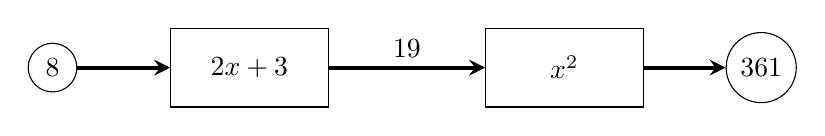
\begin{tikzpicture}[node distance = 2.5cm]
    \node (inputVal) [input] {8};
    \node (fx) [function, right of = inputVal] {$2x + 3$};
    \node (gx) [function, right of = fx, node distance = 4cm] {$x^2$};
    \node (outputVal) [input, right of = gx] {361};
    \node at (4.5,0) [anchor = south] {19};
    
    \draw [->, >=stealth, line width = 1.5] (inputVal) -- (fx);
    \draw [->, >=stealth, line width = 1.5] (fx) -- (gx);
    \draw [->, >=stealth, line width = 1.5] (gx) -- (outputVal);
    \end{tikzpicture}
\end{center}    
\end{frame}

\begin{frame}{Domain of Composition of Functions}
    The domain of the compositions of two functions $f$ and $g$ is the domain of the result \underline{before simplifying}.
\end{frame}

\begin{frame}{Example 1}
Given $f(x) =x^2-4x$, $g(x) = 2-\sqrt{x+3}$, and $h(x) = \frac{2x}{x+1}$, simplify each and find the domain of the composition. \newline\\
(a) \quad $(g\circ f)(x)$
\begin{align*}
    \onslide<2->{(g\circ f)(x) &= 2-\sqrt{({\color{red}x^2-4x})+3}} \\[8pt]
    \onslide<3->{&= 2 - \sqrt{x^2-4x+3}}
\end{align*}
\onslide<4->{Domain:
    \[x^2-4x+3 \geq 0\]}
\onslide<5->{\[x \leq 1 \text{ or } x \geq 3  \]}
\onslide<6->{\[ (-\infty, 1] \cup [3, \infty) \]}
\end{frame}

\begin{frame}{Example 1 $f(x) =x^2-4x$, $g(x) = 2-\sqrt{x+3}$, and $h(x) = \tfrac{2x}{x+1}$}
(b) \quad $(f \circ g)(x)$
\begin{align*}
    \onslide<2->{(f\circ g)(x) &= ({\color{red}2-\sqrt{x+3}})^2 - 4({\color{red}2-\sqrt{x+3}})} \\[8pt]
    \onslide<3->{&=4-4\sqrt{x+3}+\left(\sqrt{x+3}\right)^2-8+4\sqrt{x+3}} \\[8pt]
    \onslide<4->{&=4+x+3-8} \\[8pt]
    \onslide<5->{&=x-1}
\end{align*}
\onslide<6->{Domain:
\[ x + 3 \geq 0\]}
\onslide<7>{\[ [-3,\infty) \]}
\end{frame}


\begin{frame}{Example 1 $f(x) =x^2-4x$, $g(x) = 2-\sqrt{x+3}$, and $h(x) = \tfrac{2x}{x+1}$}
(c) \quad $(g \circ h)(x)$
\begin{align*}
    \onslide<2->{(g\circ h)(x) &= 2-\sqrt{{\color{red}\frac{2x}{x+1}}+3}} \\[10pt]
    \onslide<3->{&= 2 - \sqrt{\frac{2x}{x+1}+\frac{3(x+1)}{x+1}}} \\[10pt]
    \onslide<4->{&= 2-\sqrt{\frac{2x+3x+3}{x+1}}} \\[10pt]
    \onslide<5->{&= 2 = \sqrt{\frac{5x+3}{x+1}}}
\end{align*}
\end{frame}

\begin{frame}{Example 1 \quad $2-\sqrt{\tfrac{2x}{x+1}+3}$}
Domain of $(g\circ h)(x)$:
\begin{align*}
    \onslide<2->{x+1 &\neq 0} \\
    \onslide<3->{x &\neq -1}
\end{align*}
\begin{align*}
    \onslide<4->{\frac{2x}{x+1}+3 &\geq 0} \\[10pt]
    \onslide<5->{\frac{5x+3}{x+1} & \geq 0} \\[10pt]
\end{align*}
\begin{center}
    \onslide<6->{Critical values at $x = -1$ and $x = -3/5$}
\end{center}
\end{frame}

\begin{frame}{Example 1 \quad $\tfrac{5x+3}{x+1} \geq 0$}
\begin{center}
\onslide<2->{
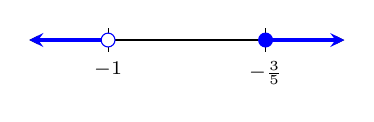
\begin{tikzpicture}
\draw[<->] (-2,0) -- (2,0);
\draw (-1,0.15) -- (-1,-0.15) node [below] {\scriptsize $-1$};
\draw (1,0.15) -- (1,-0.15) node [below] {\scriptsize $-\frac{3}{5}$};
\draw[->, very thick, blue] (-1,0) -- (-2,0);
\draw[->, very thick, blue] (1,0) -- (2,0);
\draw[color=blue, fill=white] (-1,0) circle [radius = 2.5pt];
\draw[color=blue, fill=blue] (1,0) circle [radius = 2.5pt];
\end{tikzpicture}}
\end{center}
\onslide<3->{
\[ (-\infty, -1) \cup \left[-\frac{3}{5}, \infty\right) \]}
\end{frame}


\begin{frame}{Example 1 $h(x) = \tfrac{2x}{x+1}$}
(d) \quad $(h \circ h)(x)$
\begin{align*}
    \onslide<2->{(h \circ h)(x) &= \frac{2\left({\color{red}\frac{2x}{x+1}}\right)}{{\color{red}\frac{2x}{x+1}}+1}}    \\[10pt]
    \onslide<3->{&= \frac{\frac{4x}{x+1}}{\frac{2x}{x+1}+1}}
    \onslide<4->{\left(\frac{x+1}{x+1}\right)} \\[10pt]
    \onslide<5->{&= \frac{4x}{2x+x+1}} \\[10pt]
    \onslide<6->{&= \frac{4x}{3x+1}}
\end{align*}
\end{frame}

\begin{frame}{Example 1 $h(x) = \tfrac{2x}{x+1}$}
Domain:
\begin{align*}
    \onslide<2->{x + 1 &\neq 0} \\
    \onslide<3->{x &\neq -1} 
\end{align*}
\begin{align*}
\onslide<4->{(h \circ h)(x) &= \frac{2\left({\color{red}\frac{2x}{x+1}}\right)}{{\color{red}\frac{2x}{x+1}}+1}} \\[10pt]
\onslide<5->{\frac{2x}{x+1}+1 &\neq 0} \\
\onslide<6->{\frac{2x}{x+1} &\neq -1}
\end{align*}
\end{frame}

\begin{frame}{Example 1}
\begin{align*}
    \frac{2x}{x+1} &\neq -1 \\[10pt]
    \onslide<2->{2x &\neq -1(x+1)} \\[8pt]
    \onslide<3->{2x &\neq -x - 1} \\[8pt]
    \onslide<4->{x &\neq -\frac{1}{3}}
\end{align*}
\onslide<5->{\[x \neq -1, -\frac{1}{3} \]} 
\onslide<6->{\[(-\infty, -1) \cup \left(-1, -\frac{1}{3}\right) \cup \left(-\frac{1}{3}, \infty\right)\]}
\end{frame}


\end{document}
